
%(BEGIN_QUESTION)
% Copyright 2007, Tony R. Kuphaldt, released under the Creative Commons Attribution License (v 1.0)
% This means you may do almost anything with this work of mine, so long as you give me proper credit

Examine this loop diagram for a chemical reactor heating control system, then determine how the system will respond to {\it any one} of the scenarios listed below (you choose).  Your answer should describe four parameters of the control system over time: (1) What happens to the process temperature, (2) What the operator's indication does, (3) Which direction the controller's output changes, and (4) What happens to steam flow through the control valve.

$$\includegraphics[width=15.5cm]{i02450x01.eps}$$

\noindent
{\bf Choose one!}

\begin{itemize}
\item{} Broken wire connection at TB12-11
\vskip 5pt
\item{} Short in cable 20
\vskip 5pt
\item{} Resistor fails open in analog input field termination (FTA-AI)
\vskip 5pt
\item{} Sudden influx of {\it cold} fluid into reactor
\vskip 5pt
\item{} Sudden increase in steam supply pressure and temperature
\end{itemize}

\vskip 10pt

\noindent
{\bf Determine these four system responses:}

\begin{itemize}
\item{} Process temperature response over time:
\vskip 5pt
\item{} Operator indication of process temperature over time:
\vskip 5pt
\item{} Controller output over time:
\vskip 5pt
\item{} Steam flow through control valve over time:
\end{itemize}

\underbar{file i02450}
%(END_QUESTION)





%(BEGIN_ANSWER)

This is a graded question -- no answers or hints given!

%(END_ANSWER)





%(BEGIN_NOTES)

\noindent
{\bf Broken wire connection at TB12-11}

\begin{itemize}
\item{} Process temperature response over time: {\it Remains approximately the same if controller switches to manual; will increase otherwise.}
\vskip 5pt
\item{} Operator indication of process temperature over time: {\it Falls below low-scale value.  DCS will probably indicate a failed transmitter and automatically switch control mode to ``manual.''}
\vskip 5pt
\item{} Controller output over time: {\it DCS may act to place the controller in manual.  If not, the output will increase.}
\vskip 5pt
\item{} Steam flow through control valve over time: {\it Remains the same if controller goes to manual; otherwise, steam flow will increase.}
\end{itemize}

\vskip 10pt

\noindent
{\bf Short in cable 20}

\begin{itemize}
\item{} Process temperature response over time: {\it Will decrease, because steam will shut off.}
\vskip 5pt
\item{} Operator indication of process temperature over time: {\it Indication will accurately show the decrease in process temperature.}
\vskip 5pt
\item{} Controller output over time: {\it Output will increase in a futile attempt to increase steam flow.}
\vskip 5pt
\item{} Steam flow through control valve over time: {\it Valve closes fully.}
\end{itemize}

\vskip 10pt

\noindent
{\bf Resistor fails open in analog input field termination (FTA-AI)}

\begin{itemize}
\item{} Process temperature response over time: {\it Remains approximately the same if controller switches to manual; will decrease otherwise.}
\vskip 5pt
\item{} Operator indication of process temperature over time: {\it Rises above high-scale value.  DCS will probably indicate a failed transmitter and automatically switch control mode to ``manual.''}
\vskip 5pt
\item{} Controller output over time: {\it DCS may act to place the controller in manual.  If not, the output will decrease.}
\vskip 5pt
\item{} Steam flow through control valve over time: {\it Remains the same if controller goes to manual; otherwise, steam flow will decrease.}
\end{itemize}

\vskip 10pt

\noindent
{\bf Sudden influx of {\it cold} fluid into reactor}

\begin{itemize}
\item{} Process temperature response over time: {\it Temperature will immediately fall, but then stabilize as the control system compensates.}
\vskip 5pt
\item{} Operator indication of process temperature over time: {\it Indication will accurately show the real process temperature (fall, then recover).}
\vskip 5pt
\item{} Controller output over time: {\it Output will increase to add more heat to the process.}
\vskip 5pt
\item{} Steam flow through control valve over time: {\it More steam flow over time.}
\end{itemize}

\vskip 10pt

\noindent
{\bf Sudden increase in steam supply pressure and temperature}

\begin{itemize}
\item{} Process temperature response over time: {\it Temperature will increase, but then stabilize as the control system compensates.}
\vskip 5pt
\item{} Operator indication of process temperature over time: {\it Indication will accurately show the real process temperature (spike up, then recover).}
\vskip 5pt
\item{} Controller output over time: {\it Output will decrease over time.}
\vskip 5pt
\item{} Steam flow through control valve over time: {\it If the steam pressure has increased, there will be an increase in flow followed by stabilization to the old value.  If the steam temperature has increased, the flow rate will eventually decrease as the control system compensates.}
\end{itemize}

%INDEX% Documentation, loop diagram: for a DCS loop
%INDEX% Process: steam-heated reactor vessel (generic)

%(END_NOTES)


